\section{Introduction}

\begin{frame}
  \begin{columns}
    \begin{column}{0.5\textwidth}
      There exist many approaches to modeling plasticity in the context of phase-field fracture \cite{alessi_gradient_2014, alessi_gradient_2015, alessi_coupling_2018, ambati_phase-field_2015, ambati2016phase, miehe_phase_2016, borden2016phase, borden_phase-field_2017}.
      
      \bigskip
      
      We propose a variational framework for phase-field modeling of fracture in general dissipative solids \cite{hu2021variational,talamini2021attaining}. The framework accounts for:
      \begin{itemize}
        \item inertial effects, large deformation kinematics, and newtonian viscosity;
        \item inelastic deformation and associative flow rules;
        \item rate sensitivity of plastic deformation;
        \item viscous regularization of crack propagation;
        \item thermal effects including heat conduction, heat convection, and heat generation from dissipative mechanisms.
      \end{itemize}
    \end{column}
    \begin{column}{0.5\textwidth}
      \vspace{-3em}
      \begin{figure}
        \centering
        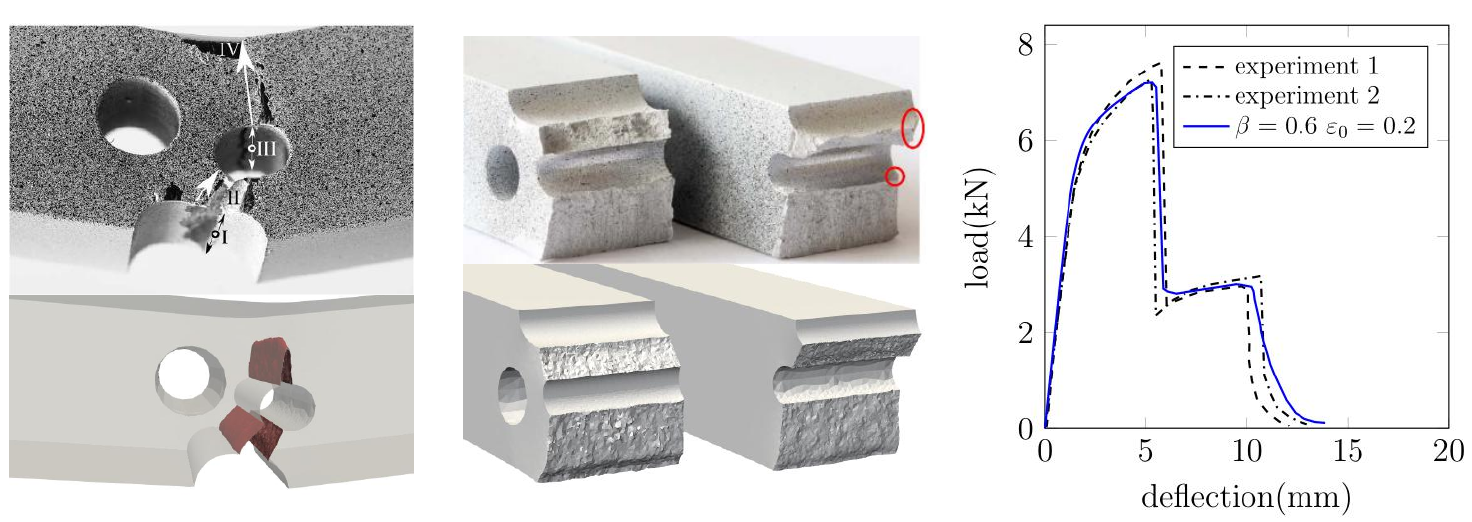
\includegraphics[width=0.83\textwidth]{introduction/figures/3pb}
        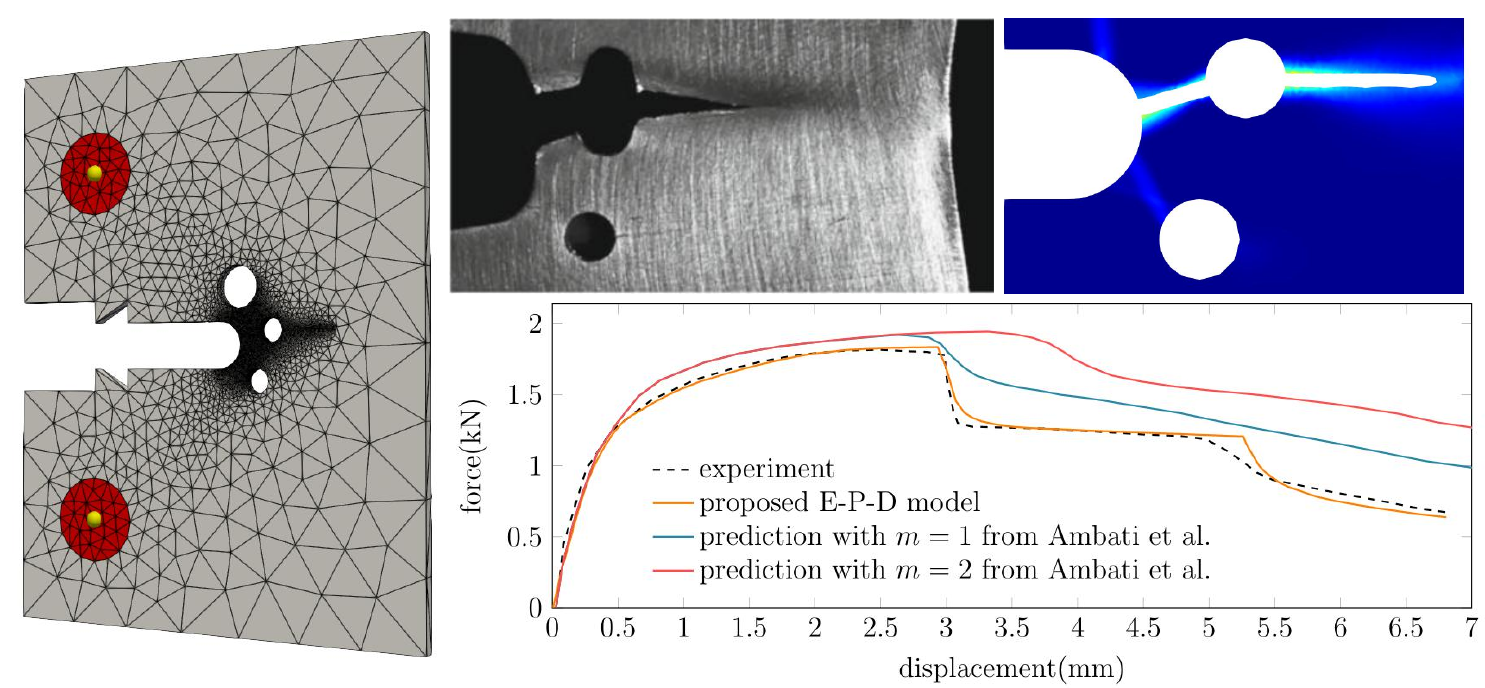
\includegraphics[width=0.83\textwidth]{introduction/figures/SFC}
        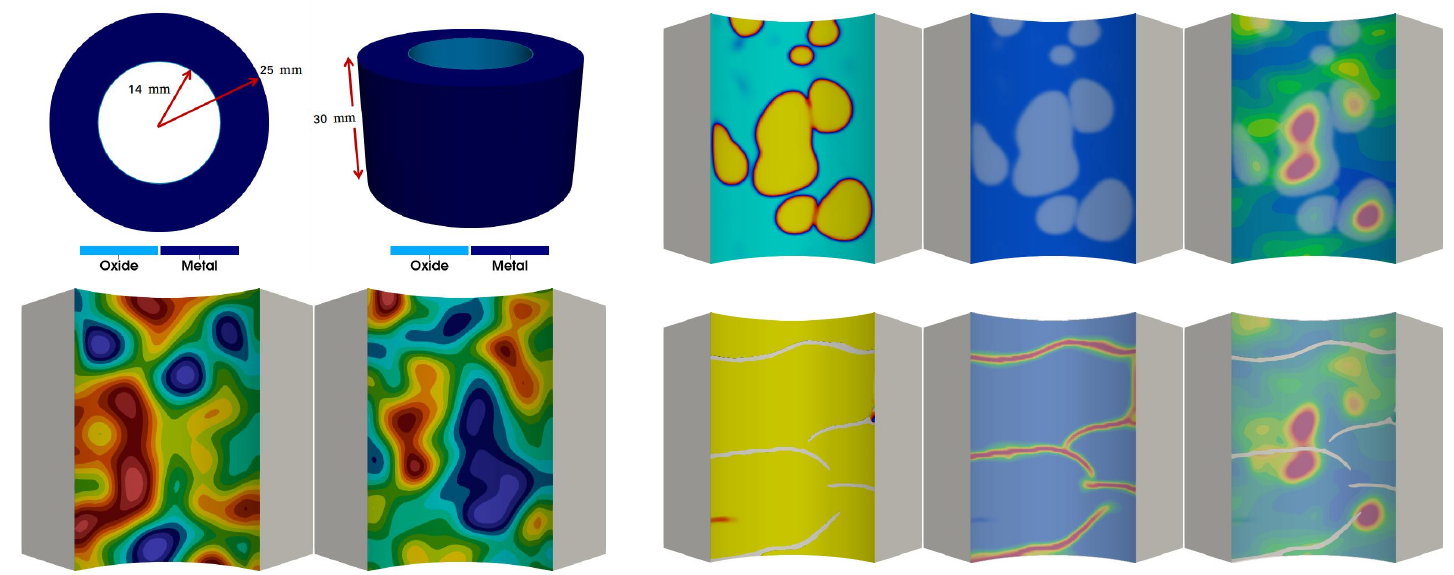
\includegraphics[width=0.83\textwidth]{introduction/figures/spallation}
      \end{figure}
    \end{column}
  \end{columns}
\end{frame}
